\section{Introduction}
\label{section:introduction}

User-friendly data analysis tools and frameworks often provide limited flexibility, as they usually focus on a predetermined set of use/analysis cases or a small fraction of the typically large data analysis pipeline. This lack of flexibility often pushes code-literate analysts towards the use of interactive notebooks such as Jupyter.

Interactive notebooks allow the use of popular, high-level and highly expressive imperative languages, such as Python, for analyzing data and composing the results into an easily readable notebook-like interface. Due to the wide popularity of such languages, there is also a huge collection of third-party libraries that can be used by data scientists as building blocks of a much bigger analytical process. Furthermore, the web environment of notebooks enables collaboration between data scientists, since it allows them to directly interact with the user interface in order to develop and run code, process data, generate visualizations, and lastly, compose their findings into an interactive (and re-runnable) report-like page, that contains code, visualizations and textual description of the analysis.

However as we show in this work, interactive notebooks are still suboptimal with regard to ease of use and interactivity. Setting up notebook environments and dependencies, obtaining and combining data and generating the respective visualizations, requires technical knowledge that often exceeds the skill-set of a typical data scientist. Lastly, while such notebooks support the generation of interactive visualizations, this interactivity is not an integral part of the data analysis process. 

We address these issues, by extending interactive notebooks with the  {\projname} framework. {\projname} notebooks support a new template language capable of facilitating common data analysis tasks. The main contributions of this extension are:

\begin{itemize}
	\item \textit{Expressive template language:} Prior work, treats a page as a database view. Building on that, our template language goes beyond SQL query and view definition in both style and fundamental expressiveness. It is a mixture of query as well as web templating language that works on ordered (arrays) and semi-ordered (JSON) data. 
	\item \textit{Easy data retrieval:} Our framework supports communication with all major database types, such as Postgress, MongoDB, SQL etc, eliminating the need for individual DB drivers. Furthermore, using {\projname}, user access credentials for the database server(s) are stored in a configuration file, eliminating the embarassingly insecure practice of typing usernames and passwords in notebook cells vidible to everyone.
	\item \textit{Inline JSON operations:} The primary data structure used in {\projname} is JSON arrays. {\projname} combines the intuitive nature of JSON with the ability to write inline JSON operations, resulting in a clean, structured and readable code.
	\item \textit{Variable binding:} Analysts can easily ``bind'' variables using our template language. ``Binding'', results in automatic re-execution of notebook cells that contain those variables upon a change. {\projname} will trigger execution of the appropriate cells without any extra coding effort. As we show later, combined with inline JSON operations, binding becomes an incredibly versatile tool.

%	\item \textit{Declarative semantics:} {\projname} implements formal declarative \textit{Model-View-View-Model} (MVVM) semantics. \remark{Fill in why this is a good thing. I have no idea.}
%	\item \textit{Expressive template language:} Prior database work, treats a page as a database view. Building on that, our template language goes beyond SQL query and view definition in both style and fundamental expressiveness. It is a mixture of query as well as web templating language that works on ordered (arrays) and semi-ordered (JSON) data. 
%	\item We allow in-line declarative code directly in JSON...
\end{itemize}

Throughout this paper, we present {\projname} via an example data analysis: We assume a scenario where a data analyst must (a) retrieve  website access information from a database, (b) plot a line chart of access count Vs timestamp, as well as a bar chart of access count Vs age groups, and (c) be able to select a time range from the line chart using mouse input and automatically filter and display data in the second plot to present age-group-based activity within the selected time frame. 

For our walkthrough example, we assume a Jupyter server where the analysts develop their notebooks and a different database server where data is stored. Table \ref{tab:schema} shows how our databases are organized. The analyst's first task is to retrieve the data via database queries, join the two tables based on the visitor id (``vid'') key and group by (1) ``time'' and (2) ``age'' to prepare the data for the two plots.

During the visualization stage, the analyst implements two ``linked'' plots in such a way that a range selection in the first plot \textit{automatically} (without re-executing code in the notebook) filters the data presented in the second plot. Figure \ref{fig:vision} illustrates the expected chart behavior. A time-frame selection in the first chart (10:00AM - 1:00PM) causes the second chart to only plot those accesses that occurred during the selected interval. 

It is important to note that this interactive chart implementation using imperative languages is not a trivial task and possibly beyond the coding skill set of an average data analyst. Such a task requires advanced coding skills and implementation of event listeners to capture the user's mouse input and asynchronously trigger execution of other functions that will update data and re-draw the second figure. As we show later in Section ??, the {\projname} framework is equipped with modules that can take care of the heavy work, while the analyst only needs to define ``bound'' (linked) variables.

\begin{table}
\begin{center}

\begin{tabular}{|c|c|c|c|}
\hline 
\multicolumn{4}{|c|}{Table name: ``page\_views''} \\ 
\hline 
page\_view\_id & v\_id & url & time \\ 
\hline 
\end{tabular} 

\hfill

\begin{tabular}{|c|c|c|c|c|}
\hline 
\multicolumn{5}{|c|}{Table name: ``visitors''} \\ 
\hline 
vid & name & lastname & username & age \\ 
\hline 
\end{tabular} 

\end{center}
\caption{Schema description of the two tables in our database.}
\label{tab:schema}
\end{table}

The remainder of this paper is organized as follows: Section ?? discusses the architecture of the {\projname} framework. Due to space limitation, we focus on those aspects that can be useful as a notebook extension. Section ?? presents our example data analysis. Finally, Section ?? concludes the paper.

\begin{figure*}
	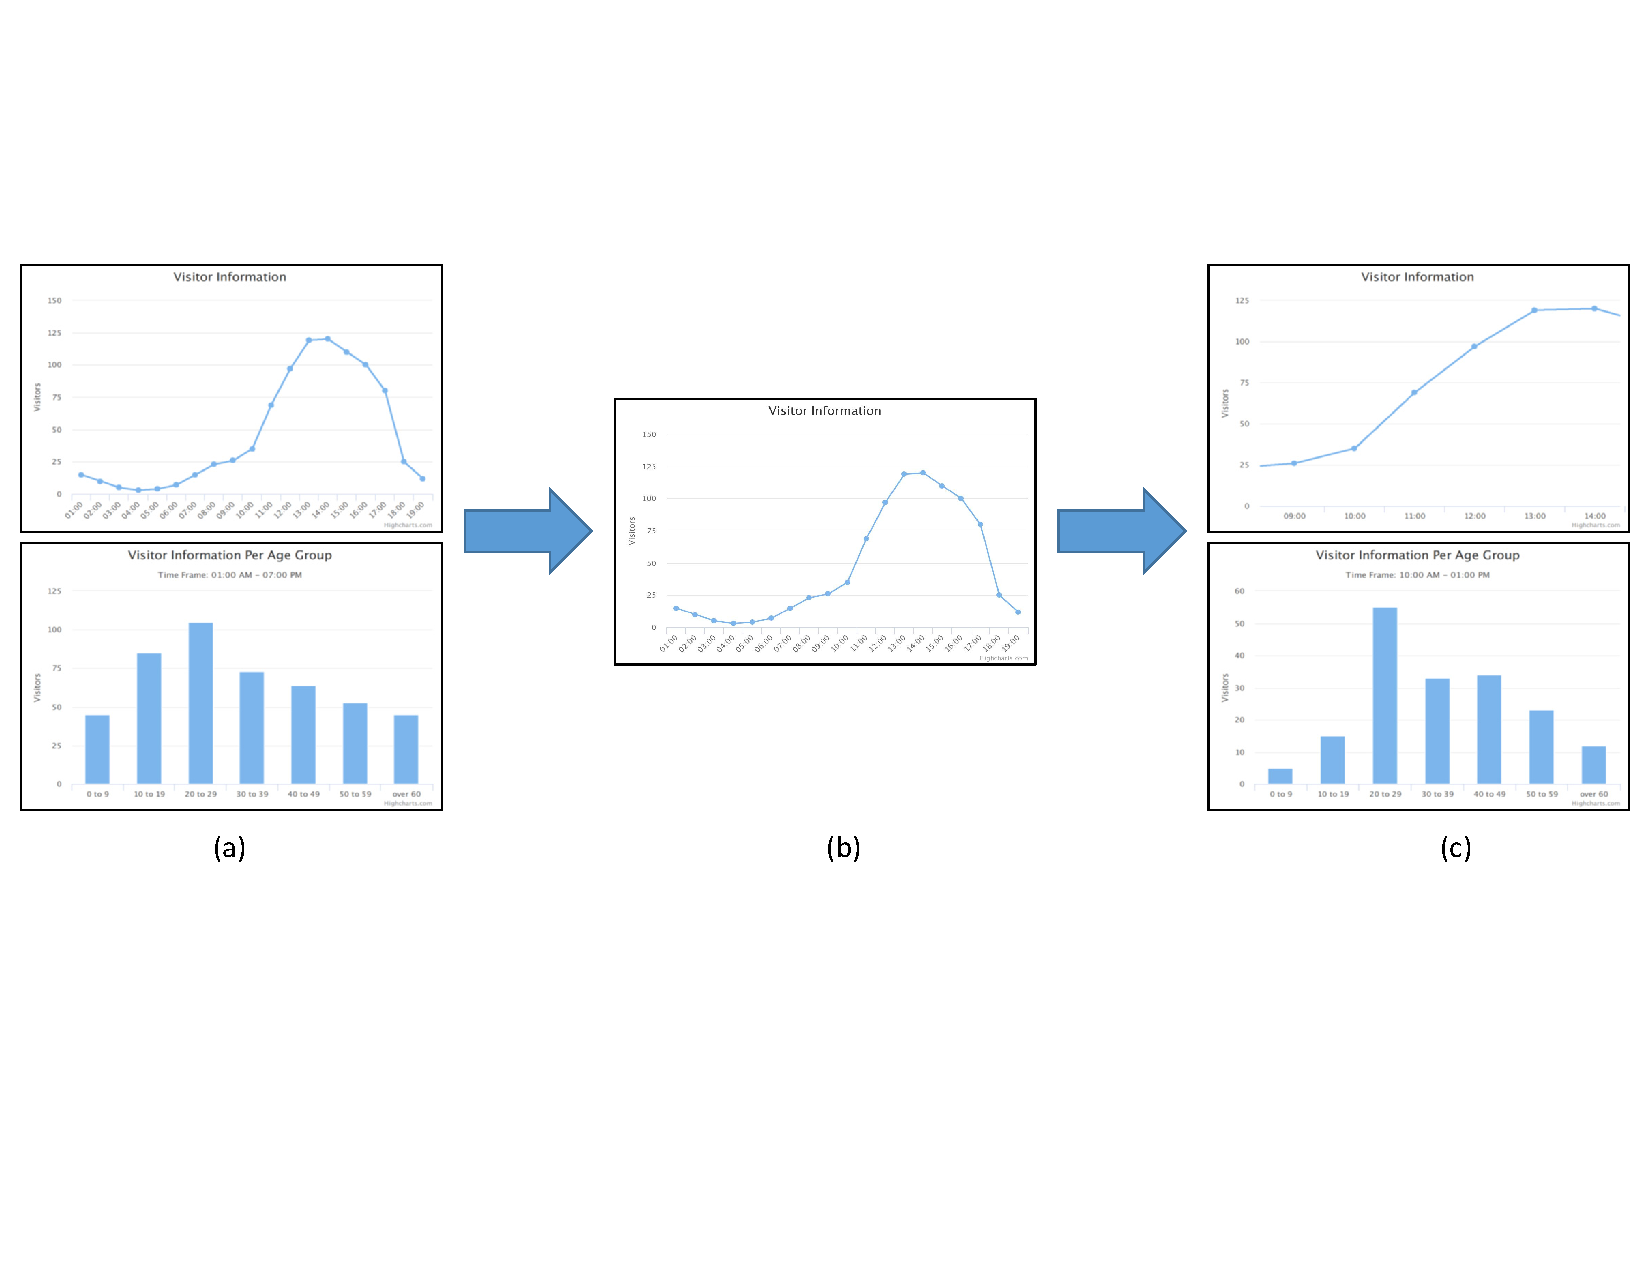
\includegraphics[width=\textwidth]{figures/highchart_final_a.pdf}
	\caption{Demonstration of interactive charts. The analyst's selection automatically updates the second plot (right).}
	\label{fig:vision}
\end{figure*}

\begin{figure*}
	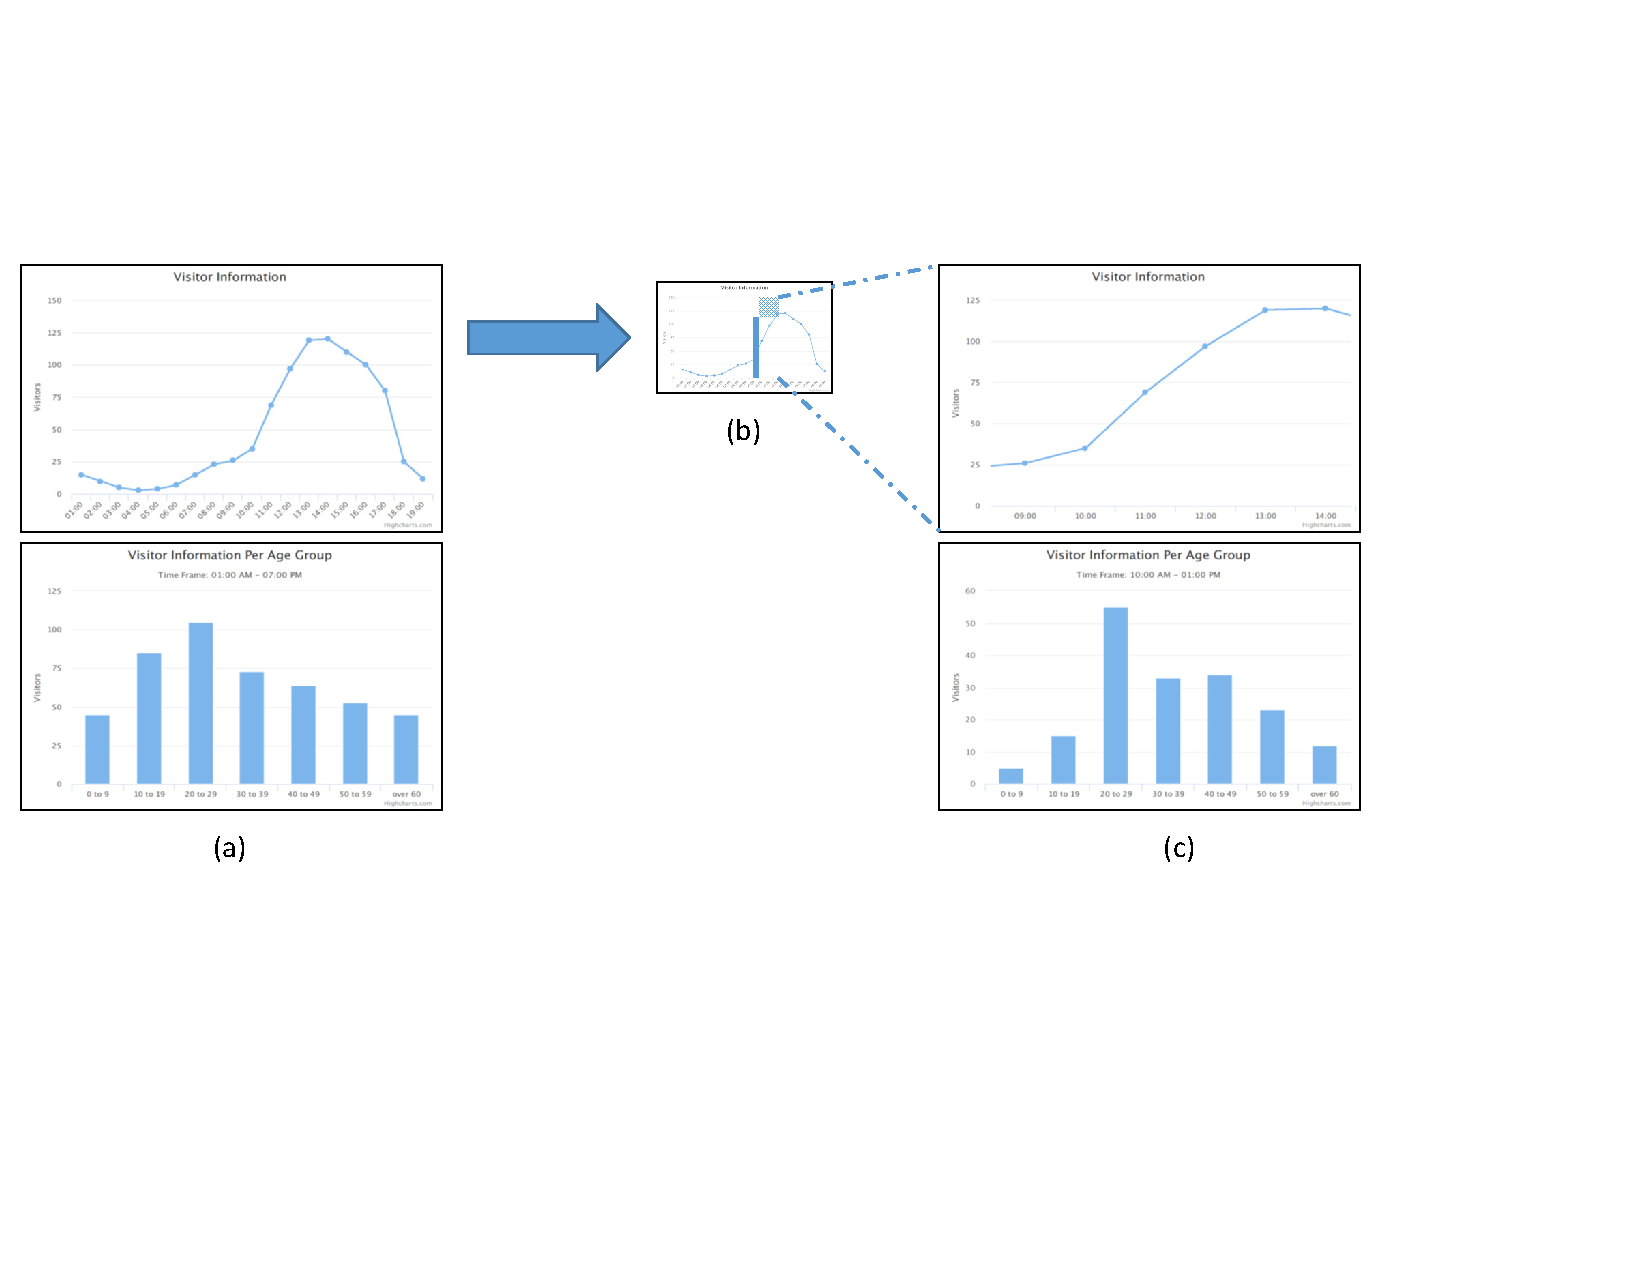
\includegraphics[width=\textwidth]{figures/highchart_final_b.pdf}
	\caption{Demonstration of interactive charts. The analyst's selection automatically updates the second plot (right).}
	\label{fig:vision}
\end{figure*}

\remark{Ok I thought about it and I propose the following modifications in the paper structure (Nothing major - just moving text around to make it more readable): We begin with a good discussion about the vidette features that can help notebooks in section 2. We then show the entire walkthrough in one section (Section 3). By now, the reader knows what vidette can do so it will be easier to follow and understand the code we show.}

%In this paper, we demonstrate the use of {\projname} via a walkthrough example. Specifically, we want to use website access data to plot an access count over time histogram. We also want to plot the recorded user demographics (with focus on age groups). We then want to have the ability to interact with the histogram plot and select a time region. This action should automatically update the second plot with the user demographics in the selected time window. 
%
%Without loss of generality, we assume a Jupyter server, where the analysts develop their notebooks and a different database server where data is stored. To retrieve the entirety of the required data, we have to query two different databases and join the returned JSON files. Figure ?? shows how our databases are organized. Our fictional analyst will perform the following high-level tasks:
%
%\begin{itemize}
%	\item Data retrieval from remote databases. 
%	\item Data curation: Join data and prepare for visualization.
%	\item Data visualization.
%\end{itemize}
%
%The remainder of this paper is organized as follows: Sections \ref{section:dataretrieval} -- \ref{section:visualization} present a direct comparison of using {\projname} and an imperative language such as Python in order to complete the tasks of our example. Throughout these sections, we demonstrate some of the main contributions of {\projname}. Section \ref{section:discussion} provides further discussion regarding our proposed extension and presents other useful aspects of it not used in our walkthrough. Finally, Section \ref{section:conclusion} concludes the paper.

